\section{Overview}
In this experiment, electrons emitted as a result of the radioactive
beta decay of \cs are measured as a function of their momentum by
deflecting them in a magnetic field. \ The resulting spectrum is
evidence for a complex decay scheme with several possible pathways.

\section{Theory}
\subsection{Beta Decay}

It is energetically favorable for stable nuclei of a given element to
have the ratio of neutrons to protons in a relatively narrow range.  A
nucleus with too many or too few neutrons will generally be unstable
and can transform into a more stable nucleus in a process known as beta
decay.  For a nucleus with an excess of neutrons the beta decay
process can be represented schematically as $n \to p + e^- + \bar{\nu}$.
Inside the nucleus, a neutron changes into a proton; in addition,
two particles are emitted from the nucleus, a beta particle [either an
electron ($e^-$) or a positron
($e^+$)---in this case an electron]
and a neutrino ($\nu$ or $\bar{\nu}$).  These particles carry
away the energy released in the decay of the original nucleus into a
more stable nucleus.

In practice, neutrinos cannot be detected with most apparatus.
On the other hand, it is straightforward to observe electrons emitted
in beta decay and to measure their speed. Examining the emitted
electrons, it is found that they possess a range of kinetic energies
from zero up to the maximum energy
$E_{\rm max}$ released in the decay process.
The broad spectrum of electron energies suggested that the energy
released in the decay was being shared by the beta particle and an
unseen companion particle.  In 1930, the physicist Wolfgang Pauli
analyzed the energy and momentum of the emitted beta particle and the
recoiling nucleus and concluded that the unseen particle (which he
named the ``neutrino'') had mass that was
very much smaller than the mass of the electron, and could be taken as
essentially equal to zero.  Direct observation of neutrinos did not
occur until several decades later.


Nuclei with an excess of protons undergo a beta decay in which a
proton is transformed into a neutron in the nucleus, and a positron
$e^+$ (the antiparticle of the
electron, with charge $+e$) and a neutrino are emitted and share the
energy released in the decay.


\subsection{Gamma Decay and Internal Conversion}


When a new nucleus is formed in a nuclear reaction such as beta decay,
the nucleus often has an excess of energy.  Using the language of
quantum mechanics, it is in an excited state.  Typically, such a
nucleus will then make a transition to the lowest-energy state  (or
ground state) while emitting a photon, which carries away the excess
energy.  These emitted photons have high energy and therefore very
short wavelength, and are called gamma rays.


In the radioactive decay to be studied in this experiment, gamma
rays (photons) are in fact produced.  However, we cannot observe these
photons directly in our beta spectrometer---it can only detect charged
particles such as electrons or positrons.  However, we
{\em can} detect the gamma rays photons indirectly, via a
process called {\bf internal conversion}.  When a nucleus
emits a photon, there is some probability that the photon will interact with and
be absorbed by one of the electrons surrounding the nucleus.  The
probability is largest for the K-shell electrons---which form the
innermost shell and are closest to the nucleus.  The probability is
smaller for electrons in the L and higher-energy shells.  The net
effect is that a gamma ray photon is
``converted'' into an emitted electron.
 These converted electrons all have a definite energy---equal to the
gamma ray energy minus the energy required for the electron to escape
from the atom.  The converted K electrons are the most numerous, and
also have the lowest energy, since more energy is required for them to
escape the nucleus.  These electrons will produce a large, sharp
peak in the spectrum of emitted electrons.  The converted L electrons
will produce a smaller peak and at slightly higher energy than the K
electrons, etc.


\subsection{\cs Decay Scheme}


\bigskip

The isotope of cesium,
\cs
(also written as Cs-137) has an interesting decay scheme.  As shown in
Figure~\ref{fig:csdecay} below, \cs can decay directly to
${}^{137}_{56}{\rm Ba}$
\begin{figure}
\begin{centering}
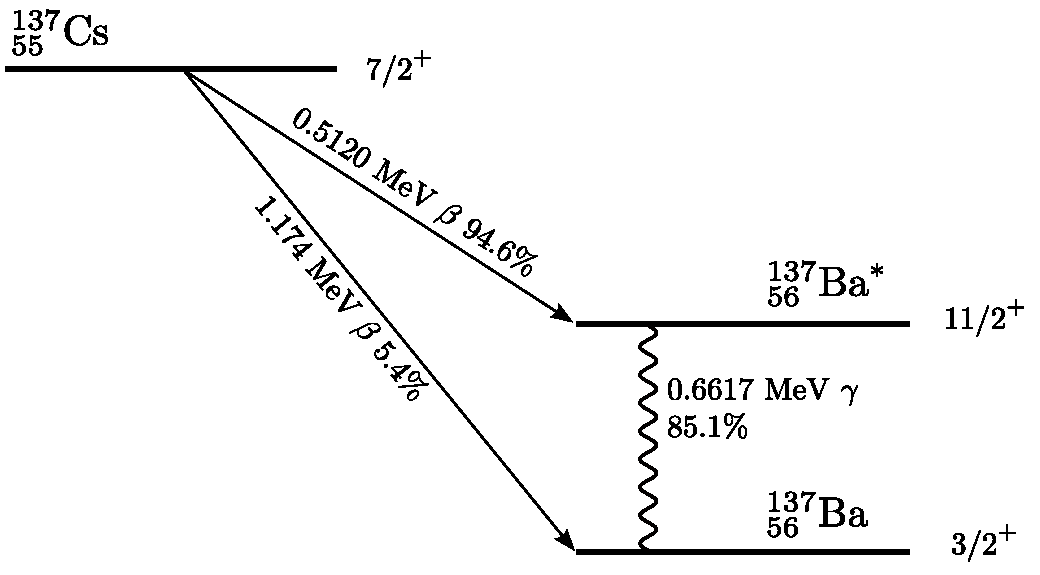
\includegraphics[width=4.1661in,height=2.1661in]{../images/Cs-137-decay.pdf}
\caption{ \cs decay scheme.  Decay energies listed are accepted values. }
\label{fig:csdecay}
\end{centering}
\end{figure}
via beta decay, releasing an energy of 1.18 MeV.  However, only 8 \%
of the decays proceed that way.  The great majority of the \cs
nuclei decay in a two step process, first with a beta decay to ${}^{137}_{56}{\rm Ba}^*$,
which is an excited state of
${}^{137}_{56}{\rm Ba}$.
This decay releases energy 0.512 MeV, which is shared between an
emitted electron and a neutrino. In the second step, the ${}^{137}_{56}{\rm Ba}^*$ makes
a transition to the ground state, ${}^{137}_{56}{\rm Ba}$ by emitting a gamma ray photon
of energy 0.662 MeV.  Some of these photons are internally
converted---absorbed by an inner shell electron.  These electrons are
then emitted with energy approximately equal to 0.662 MeV
(actually slightly less, since some of the absorbed energy is used in
the process of the electron escaping from the ${}^{137}_{56}{\rm Ba}$ atom).

In this experiment, we observe the electrons emitted in the beta
decay from \cs to ${}^{137}_{56}{\rm Ba}^*$.  These electrons have kinetic energy
$E_{\rm K}$ ranging from zero to a maximum 
$E_{\rm Km} = 0.512 {\rm MeV}$, the energy released
in the decay.  We also observe the internally converted electrons,
which have kinetic energy approximately equal to
$E_{Kc} = 0.662 {\rm MeV}$.  If one plots the
number of electrons emitted by \cs as a function of their kinetic
energy, one expects a plot that is illustrated schematically in Fig.~\ref{fig:Espectrum}
below.  The broad peak is from the electrons emitted by beta decay of
\cs to \bam;  the narrow peak is from the electrons internally
converted from the gamma ray photons emitted in the decay from \bam
to \ba.  In this figure, we have neglected the 8 \% of the electrons emitted 
in the direct beta decay from \cs to \ba.
\begin{figure}
\begin{centering}
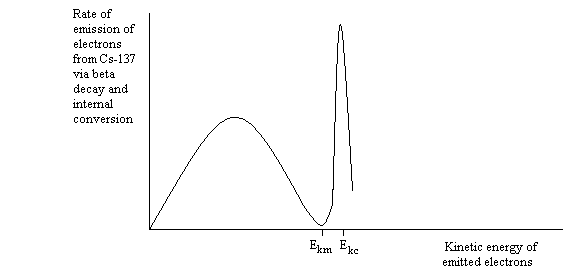
\includegraphics[width=5.889in,height=2.8189in]{../images/beta-img2.png} 
\caption{Schematic spectrum of electrons emitted from \cs}
\label{fig:Espectrum}
\end{centering}
\end{figure}

\subsection{Beta spectrum, Kurie Plot}

The quantitative description of the beta decay spectrum is based on the
following relations:

\begin{equation}
R~=~A(E_{\rm m} - E)^2p^2~=~A(E_{\rm Km} - E_{\rm K})^2p^2
\label{eq:1}
\end{equation}

\begin{equation}
p~=~e B r
\label{eq:2}
\end{equation}

\begin{equation}
E~=~mc^2 + E_{\rm K}
\label{eq:3}
\end{equation}

\begin{equation}
E^2~=~p^2c^2 + m^2c^4
\label{eq:4}
\end{equation}

where:

\begin{description}
\item[$R$] = the number of electrons (or positrons) emitted per unit time in the beta decay process

\item[$p$] = momentum of an emitted electron (or positron)

\item[$E$] = total energy of an emitted electron

\item[$E_{m}$] = maximum total energy of an emitted electron

\item[$E_{\rm K}$] = kinetic energy of an emitted electron

\item[$E_{\rm Km}$] = maximum kinetic energy of an emitted electron

\item[$B$] = magnitude of the uniform magnetic field in the beta spectrometer

\item[$r$] = radius of the circular path traveled by the electrons in the magnetic field B

\item[$e$] = magnitude of the charge on an electron

\item[$m$] = mass of electron

\item[$A$] is a constant.
\end{description}

Eq.~\ref{eq:1} is a result obtained from the quantum mechanical theory of beta
decay.  The second equality in Eq.~\ref{eq:1} is obtained by using Eq.~\ref{eq:3}.
Eqs.~\ref{eq:3} and~\ref{eq:4} are familiar equations from special relativity
describing the motion of a particle traveling at a speed that is an
appreciable fraction of the speed of light.

Eq.~\ref{eq:2} applies to an electron of momentum $p$ traveling
perpendicular to a uniform magnetic field of strength $B$.  If the
electron is non-relativistic (with $v \ll c$), we can
apply Newton's $2^{\rm nd}$
law as follows.  The magnetic force on the electron
$\vec{F}_B$ is
given by:

\begin{equation}
\vec{F}_B~=~ - e \vec{v} \times \vec{B}
\end{equation}

and by Newton's second law,

\begin{equation}
\vec{F}_B~=~ m \vec{a} ~=~ - e \vec{v} \times \vec{B}
\label{eq:fma}
\end{equation}

The last equality in Eq.~\ref{eq:fma} implies that $\vec{a}$ is
perpendicular to $\vec{v}$, which means
that the electron travels in a circle at constant speed with
acceleration equal in magnitude to $a = v^2/r$.
Therefore,

\begin{equation}
evB~=~mv^2/r
\end{equation}
or
\begin{equation}
p~=~mv~=~eBr
\end{equation}

This proves Eq.~\ref{eq:2} for non-relativistic electrons.  It can be
shown (see Appendix) that Eq.~\ref{eq:2} also holds for relativistic electrons
(with $v < c$  and $v \approx c$).

In Eq.~\ref{eq:1}, while the electron kinetic energy
$E_K$ varies over its range, from 0 to
$E_{\rm Km}$, the electron  momentum
increases steadily from 0 to some maximum value.  Examination of Eq.~\ref{eq:1}
shows that a plot of the number of beta decays/second = $R$, plotted
as a function of $E_K$ or of $p$, should
have a single peak, approximately in the middle of the range of
$E_K$ or of $p$.  This is illustrated in
Fig.~\ref{fig:Espectrum} (the broad-peaked part of the graph).  In practice, we plot $R$
as a function of the electromagnet current $I$; this gives the same shape
curve, since $p$ is directly proportional to $B$, which is (to a good
approximation) directly proportional to $I$.

In order to test the beta decay theory quantitatively, we combine Eqs.~\ref{eq:1} and~\ref{eq:2}
to obtain the result (see Preliminary Question 2)

\begin{equation}
{\sqrt{R} \over B}~=~A^\prime (E_{\rm Km} - E_{\rm K})
\label{eq:kurie}
\end{equation}

where $A^\prime$ is a constant.  This means that if we
plot $\sqrt{R}/B$ vs $E_{\rm K}$, we should obtain a straight line
with negative slope and which intersects the horizontal axis at
$E_{\rm K} = E_{\rm Km}$.  This graph is called a Kurie
plot, and allows one to determine $E_{\rm Km}$, the energy released in the beta decay.

\section{Preliminary Questions}
\begin{enumerate}
\item Eq.~\ref{eq:2} can be evaluated directly in a consistent set of units,
such as SI units.  However, for this experiment it is convenient to
adapt Eq.~\ref{eq:2} so that the momentum $p$ is expressed in units of ${\rm MeV}/c$.

Use the standard value of $e$ and perform the appropriate unit conversions
to show that Eq.~\ref{eq:2} can be written as:
\begin{equation}
p~{\rm [MeV/c]} ~=~ 300 B~{\rm [T]}~r~{\rm [m]}
\end{equation}
or
\begin{equation}
pc~{\rm [MeV]} ~=~ 300 B~{\rm [T]}~r~{\rm [m]}
\end{equation}

Note: $1 {\rm MeV} = 10^6 {\rm eV}$.

Hint: Start with Eq.~\ref{eq:2} and show that if $B = 1.0 {\rm T}$ and $r = 1.0 {\rm m}$, then
$pc =  3.0 \times 10^8 {\rm eV} = 300 {\rm MeV}$.  Hence, show that
$pc~{\rm [MeV]} ~=~ 300 B~{\rm [T]}~r~{\rm [m]}$.

\item Combine Eqs.~\ref{eq:1} and~\ref{eq:2} to obtain Eq.~\ref{eq:kurie}, which is the basis of
the Kurie plot.

\end{enumerate}


\section{Equipment}
Beta spectrometer, vacuum pump, \cs source, Geiger-Muller
(G-M) tube, scalar.

\subsection{Notes on Equipment}

The beta spectrometer consists of a steel chamber in the shape of a
rectangular solid.  The chamber is mounted between the poles of an
electromagnet, which produces a uniform horizontal magnetic field
inside the chamber.  There are three openings into the front of the
chamber. The bottom one is for the \cs source, and the top one is
for the G-M tube which detects the emitted electrons.  The path of the
electrons which enter the G-M tube lies in a plane perpendicular to the
magnetic field direction, as shown in Figure~\ref{fig:chamber} below.  The distance
between the upper and lower port is 3.0 inches, and we see from the
figure that the radius $r$ of the circular path followed by the electrons
must be $3.0~{\rm inches}/2 = 1.5~{\rm inches} =  0.0381~{\rm m}$.

\begin{figure}
\begin{centering}
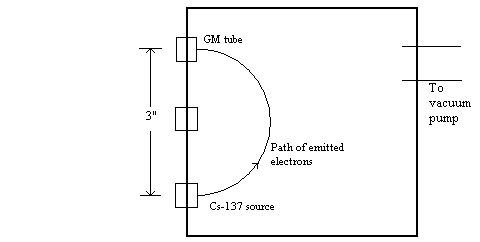
\includegraphics[width=4.9992in,height=2.528in]{../images/beta-img5.png} 
\caption{Beta spectrometer chamber.  Magnetic field is perpendicular to the plane of the figure.}
\label{fig:chamber}
\end{centering}
\end{figure}

Energetic electrons travel only a few cm in air, due to collisions with
air molecules.  In order to detect a significant fraction of the
electrons emitted by the \cs source, the spectrometer chamber is
evacuated with a vacuum pump.

\section{Procedure}

Initially, we carry out a preliminary step.  We use the gaussmeter
to measure the magnetic field produced in the beta spectrometer, as a
function of the electromagnet current (part A).  After this step, we
determine the Geiger-Muller (G-M) tube plateau and the background count
(part B), and finally, measure the spectrum of electrons emitted from
\cs (part C).

\subsection{A. Calibration curve for the electromagnet}

Note: In the measurement done with the gaussmeter, the flat side of the
gaussmeter probe must be oriented perpendicular to the direction of the
magnetic field.  You can check the orientation by rotating the probe
slightly.  In the proper orientation, the gaussmeter reading will be
at a maximum.

The magnetic field in the spectrometer is measured by inserting the
gaussmeter probe in the center port of the spectrometer.

\begin{enumerate}
\item Adjust the electromagnet current $I$ in steps of 0.10 A, from 0 to
1.50 A.  Measure the magnetic field $B$ for each value of $I$.  After the
measurements are complete, replace the cover on the center port.

\item Tabulate the values of $I$ and the corresponding measured
values of $B$.  Express $B$ in Tesla (the SI unit).  Recall that 
$1 {\rm T } ~=~ 10^4 {\rm G} = 10 {\rm kG}$.  Plot a graph of $B$
vs $I$.  Do a curve fit which expresses $B$ as a function of $I$.  This
will be your calibration curve for the electromagnet.

\item Set the electromagnet current at 0.50 A.  Use a compass
to determine the direction of the magnetic field
$\vec{B}$ in the immediate vicinity of the beta
spectrometer.  Assume that the \cs sample will be located in the
lower port of the spectrometer, and the detector---a G-M tube---will 
be in the upper port.  Sketch the path that the electrons follow
from source to detector, and include the direction of
$\vec{B}$ in your sketch.  Use the right-hand rule
for magnetic force to determine the predicted direction of the force on
the electrons after they are emitted by the \cs.  Is the predicted
direction of the force correct in order for
the electrons to be deflected toward the detector (the G-M tube)?
Explain briefly, referring to your sketch.

\end{enumerate}

\subsection{B.  G-M tube characteristics and background count rate}

{\bf CAUTION}: The instructor will handle and
position the \cs source.  This source is in the form of a powder on
a thin membrane surface, and is therefore delicate and easily
disturbed.  Contamination is a concern.  {\bf Students must not handle the
\cs source}.

\begin{enumerate}
\item The instructor will mount the G-M tube over the \cs source.

\item Measure the number of counts in a 30 second time interval as the
tube voltage is varied from 0 to 620 volts.  Increase the voltage in
increments of 50 volts until you begin to record counts.  After counts
appear, reduce the voltage increment to 20 volts. {\bf Do not exceed 650
volts!}

\item Sketch a graph of counts/30 second interval as a function of tube
voltage.  Determine a suitable plateau voltage and set the tube
voltage to that value for the reminder of the experiment. 
Include this graph with the data for this experiment.

\item The instructor will place the \cs source and the G-M tube in
the appropriate openings in the spectrometer chamber, and then turn on
the vacuum pump.  If, after a few seconds, the pump makes relatively
soft clicking sounds, the vacuum inside the spectrometer chamber should
be acceptable.  If the pump makes relatively loud gurgling sounds,
then the vacuum seal of one or more of the spectrometer ports is
inadequate.  In this event, the pump should be shut off and the seals
rechecked.

\item With the source in the spectrometer chamber under vacuum but no
magnetic field, measure the background count for 10 minutes.

\end{enumerate}

\subsection{C.  Beta spectrum and internal conversion peaks}

\begin{enumerate}

\item With vacuum in chamber, measure counts for 2.0 minute intervals.
Increase the electromagnet current $I$ starting from zero in steps of
0.10 Amps.  Do not exceed 1.50 Amps.

Refer to the schematic plot of Fig.~\ref{fig:Espectrum}.  Note that after the broad beta
decay peak, a much sharper internal conversion peak should appear.
For measurements in the vicinity of the internal conversion peak, use
smaller electromagnet current steps, {\em e.g.}, 0.05 Amps.

\item After the first sharp internal conversion peak, there should be a
second, smaller peak at slightly higher values of $I$ (see discussion in
the Theory section, under Internal Conversion).  Continue to increase
$I$ by small increments to see if you can detect it.

\end{enumerate}

\section{Analysis}

\begin{enumerate}

\item Subtract the background count rate (Procedure B5) from the count
rate data (Procedure C1 \& C2) to yield the emitted-electron count rate
$R$.  Be sure to use a consistent set of units (e.g. counts/minute).

\item Plot carefully $R$ vs electromagnet current $I$.

\item Tabulate for the beta decay count data (which gives the
broad peak) the following quantities for each value of electromagnet
current I for which counts were measured.  Do {\em not}
include in this table the count data taken around the (narrow) internal
conversion peak.

\begin{tabular}{c c c c c c}
$I$ & $R$ & $B$ & $p$ & $E$ & $E_{\rm K}$\\
\end{tabular}

Notes:
\begin{enumerate}
\item The first three quantities are obtained directly from your count
data corrected for background (Analysis step 1) and your electromagnet
calibration curve (Procedure step A2).

\item The remaining three quantities refer to the beta decay electron,
and are calculated as follows:  First find the electron momentum $p$ from the magnetic field $B$,
using Eq.~\ref{eq:2}.  Then use Eqs.~\ref{eq:3} and~\ref{eq:4} to find $E$ and, finally,
$E_{\rm K}$.

\item It is convenient in these calculations to express all
energies in units of MeV and to express the momentum $p$ in MeV/c.  The
result of Preliminary Question 1 will be helpful here.  Also, recall
that the rest energy of the electron, $mc^2 = 0.511 {\rm MeV}$.
\end{enumerate}

\item (Kurie plot).  The theoretical prediction for the beta
decay counting rate is given by Eq.~\ref{eq:1}.  In the Theory section and
Preliminary Question 2 it was shown that Eqs.~\ref{eq:1} and~\ref{eq:2} could be
combined  to yield Eq.~\ref{eq:kurie}, which provides a straightforward test of
the theory.  If the count rate data obey Eq.~\ref{eq:1}, then a plot of
$\sqrt{R}/B$ vs $E_{\rm K}$ should yield a straight line.

Using the values tabulated in step 5 above, plot
$\sqrt{R}/B$ vs $E_{\rm K}$.  Comment on the shape of the
graph.

Use the graph to determine $E_{\rm Km}$, the maximum
kinetic energy of an electron emitted in the beta decay.
Hint:  See the discussion just preceding and following Eq.~\ref{eq:kurie}.

\item In the Theory section it was claimed that, in a beta decay
process, the maximum kinetic energy of an emitted electron was equal to
the energy released in the decay.  See the text just preceding and
following Fig.~\ref{fig:csdecay}.

Compare your experimental value of
$E_{\rm Km}$ found in step 4 above to the
accepted value of the energy released in the beta decay of \cs to
\bam (see the \cs decay scheme in Fig.~\ref{fig:csdecay}).

\item Find the current at which the narrow internal conversion
peak occurs.  From your electromagnet calibration curve (or the
curve-fit function), determine the corresponding value of the magnetic
field $B$.  Using that value of $B$, calculate the total energy
$E_{\rm c}$ for an internally converted
electron emitted at the internal conversion peak.  From this, compute
the kinetic energy $E_{\rm Kc}$ of the
electron.  Use the same method of calculation as described in the
Notes for Analysis step 3 above.

\item Explain qualitatively the physical origin of the internal
conversion electrons.  In the decay scheme shown in Fig.~\ref{fig:csdecay}, which
energy should approximately equal $E_{\rm Kc}$?
Explain briefly.  Compare your experimentally-determined value of
$E_{\rm Kc}$ (from step 6 above) to the
appropriate energy value given in the decay scheme.
\end{enumerate}

\section{Appendix}
Derivation of Eq.~\ref{eq:2} for an electron moving at
relativistic speed.

In relativistic mechanics, Newton's
$2^{\rm nd}$ law is replaced by
\begin{equation}
\vec{F}_B ~=~ {d\vec{p} \over dt} ~=~ -e \vec{v} \times \vec{B}
\end{equation}
for an electron
moving  in a uniform magnetic field. We note that $\vec{F}_B \cdot \vec{v} ~=~ 0$,
since the cross product $\vec{v} \times \vec{B}$
is perpendicular to $\vec{v}$.

Now recall that the change in relativistic kinetic energy of a
particle is defined to be equal to the work done by the net force on
the object.  The work done in time $dt$ is just
\begin{equation}
dW ~=~ \vec{F}_B \cdot d\vec{r} ~=~ \vec{F}_B \cdot \vec{v} dt
\end{equation}
and this in turn is equal to the change in kinetic energy
$dE_{\rm K}$.  Therefore, we have the
familiar result,
\begin{equation}
\vec{F}_B \cdot \vec{v} ~=~ {dE_{\rm K} \over dt}
\end{equation}
However, since $\vec{F}_B \cdot \vec{v} = 0$
in this case, it follows that the electron's kinetic
energy $E_{\rm K}$ is constant.  It then
follows from Eqs~\ref{eq:3} and~\ref{eq:4} that the total energy $E$ and the magnitude
$p$ of the electron momentum are themselves constant.  Since the
relativistic momentum $p$ defined as
\begin{equation}
\vec{p} ~=~\gamma m \vec{v}
\end{equation}
and has a constant magnitude, we see that the magnitude of the
electron velocity $\vec{v}$ must also be constant.
Hence, the relativistic counterpart of Newton's
$2^{\rm nd}$ law becomes:
\begin{equation}
\vec{F}_B ~=~ {d\vec{p} \over dt} ~=~ \gamma m \vec{a} = -e \vec{v} \times \vec{B}
\end{equation}
since $v$ is constant. Note that this equation is the same
as Eq.~\ref{eq:fma}, except that the mass $m$ is replaced by $\gamma m$.
Hence, we conclude, as in the non-relativistic case, that
$\vec{a}$ is perpendicular to
$\vec{v}$ and the electron's motion
is circular.  Following the steps following Eq.~\ref{eq:fma}, we
again arrive at Eq.~\ref{eq:2}, $p = eBr$, except that $p$ is now the magnitude
of the {\em relativistic} momentum.

\section{References}
\begin{enumerate}
\item Tipler and Llewellyn, Modern Physics, $5^{\rm th}$ ed., pp. 499-501, 504-505
\end{enumerate}

\end{document}
